\begin{frame}{How can we retrieve these features?}
    \begin{tikzpicture}
        \node[] at (-5.25, -3.5) {};
        \node[] at (5.25, 3.5) {};

        \visible<1>{
            \node[anchor=north, font=\Large\bfseries] at (0, 3.5) {
                Activation maximization
            };
            \node[inner sep=0pt, draw=black, label=below:\tiny{\url{https://www.tensorflow.org/tutorials/generative/deepdream}}] at (0, 0) {
                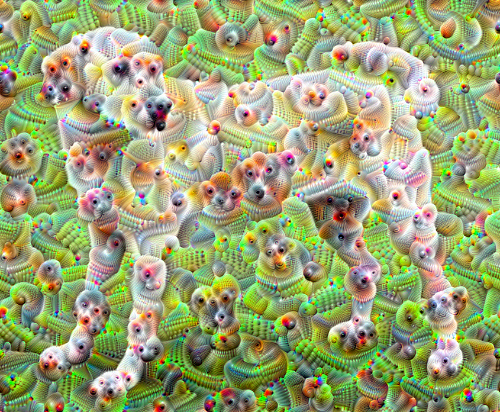
\includegraphics[width=6cm]{data/dogception.png}
            };
        }
        \visible<2>{
            \node[anchor=north, font=\Large\bfseries] at (0, 3.5) {
                Saliency mapping
            };
            \node[inner sep=0pt, draw=black] at (0, 0) {
                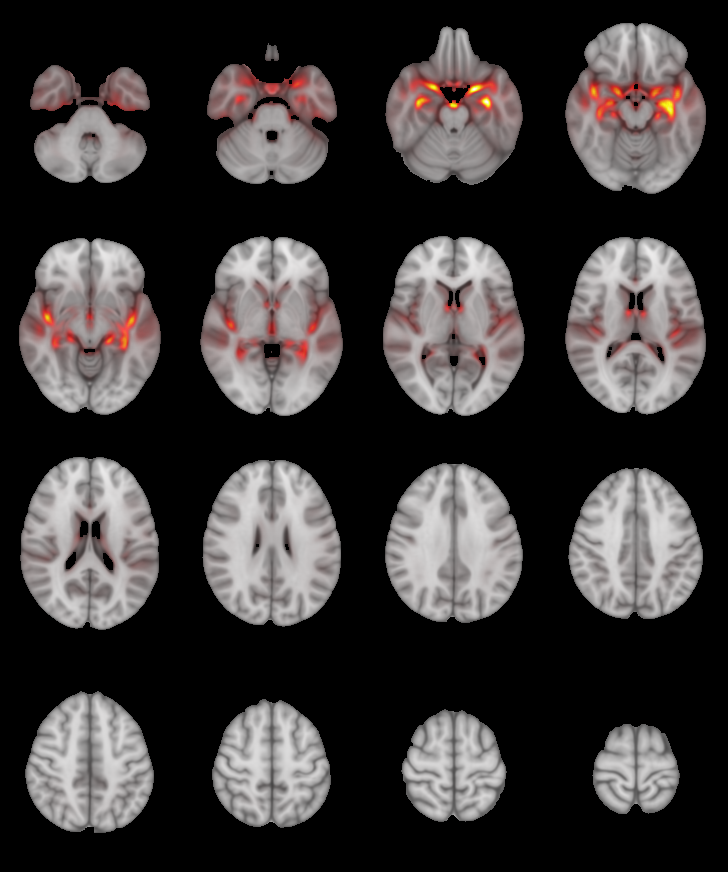
\includegraphics[width=4cm]{data/dementia.png}
            };
        }
        \visible<3>{
            \node[anchor=north, font=\Large\bfseries] at (0, 3.5) {
                Concept discovery
            };
            \node[inner sep=0pt, draw=black] at (-2.5, 0) {
                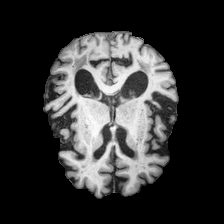
\includegraphics[width=4cm]{data/mri_axial.png}
            };
            \node[draw=black, text width=4cm, align=flush left] at (2.5, 0) {
                The patient shows widespread \textcolor{red}{cortical atrophy} and \textcolor{red}{reduced hippocampal volumes} in addition to \textcolor{red}{enlarged ventricles} and \textcolor{red}{cerebral amyloid angiopathy}.
            };
        }
    \end{tikzpicture}
\end{frame}
